The history of AI is marked by vacillations between two paradigms: the biological and the ideal one. The biological school of thought subsumes ideas like connectionism, which envisions the mind as an interconnected system of simple components, generally single neurons, and tries to build AIs via neural networks. Opposed to this view stand those schools that view the mind as an abstract machine: computationalism holds it to be an information processing system that deals in the manipulation of symbols, and which possesses structures like subsystems, rules, and syntax.

In this work, we shall build upon this latter, computationalist approach and, more specifically, upon the work of Marvin Minsky and Aaron Sloman, who have very much advocated the idea of the mind as a control system with an intelligible structure in books like {\em The Emotion Machine} \cite{emotionMachine}, {\em Society of Mind} \cite{societyOfMind}, {\em The Mind as a Control System} \cite{sloman1993}, and {\em What Sort of Control System Is Able to Have a Personality?} \cite{sloman1997}. One of the running themes in Minsky's and Sloman's work is the criterion of evolvability: it is not sufficient, they argue, to merely propose some ideal reasoning apparatus; if artificial intelligences faithful to their biological inspirations are to be constructed, we must structure them as biological minds are structured --- and that is best accomplished by thinking about what sorts of subsystems might have evolved in what order, in what way, and for what task. The human-level AI must therefore replicate the brain's functions, warts included.

In the rest of this thesis, we shall pursue this idea, with special attention given to the interaction between emotions and reasoning in the sense of logical deduction. The result will be a small cognitive architecture that combines both, but privileging neither. Both Sloman and Minsky have sketched such architectures in the past, and ours will be similar to these in its broad outlines; however, we will focus on two specific issues:

\begin{enumerate}
	\item first: \emph{how} how might certain subsystems have evolved? In what order capabilities did like pain, anger, deduction, or introspection come about and were they simply re-purposed from other, existing components, or were they created, so to speak, from scratch?
	\item Second, we look at the interactions between subsystems. How could, in evolutionary terms, something like a discrete subsystem, develop? In what manner do different subsystems in the brain communicate? Is there some universal, perhaps symbolic, communication protocol --- or a suite of protocols?
\end{enumerate}

These are deep and open questions and we will not purport to conclusively answer them here, but we will make certain educated guesses based on knowledge from neurology and evolutionary biology and these guesses will, in turn, inform the architecture of our toy artificial intelligence.

\paragraph{White-box model.} The discussion of the first issue --- the ``how'' of the evolution of subsystems --- will make up the first part of the thesis, wherein we give a possible description of the brain as an entity that evolved its capabilities in a somewhat haphazard fashion, adding new features whenever doing so was beneficial in evolutionary terms. The resultant structure of today might thus be described as somewhat haphazard (Cf. \cite[Section ``Mammalian Brain Regions'']{handbookBrainTheory}). Although it evidently possesses large-scale structure, its computational model of massively connected neurons is very different than the ones present in man-made programming languages \cite[Section ``Introducing the Neuron'']{handbookBrainTheory}. The concept we shall sketch --- and, though based on knowledge from neurology, the idea is our own --- is that of a \emph{white-box model of cognition}. Conventional structural programming models programs via functions and procedures that work as black boxes, which are called and return an answer without their caller being aware of their internal workings; we propose that one might gain some useful insights by conceiving of the brain as a collection of white boxes, wherein components can interact with and observe each other's functioning. The reasoning behind this notion is that, in a massively interconnected system such as the brain, there are no strict boundaries between parts that would be analogous to the narrow interaction between a function and its caller in a computer program; rather, typical neurons have one axon that branches into thousands of synapses that connect to other neurons \cite[p.\ 4]{handbookBrainTheory} and can, moreover, make new connections to other neurons at any time.

\begin{figure}
	\centering
	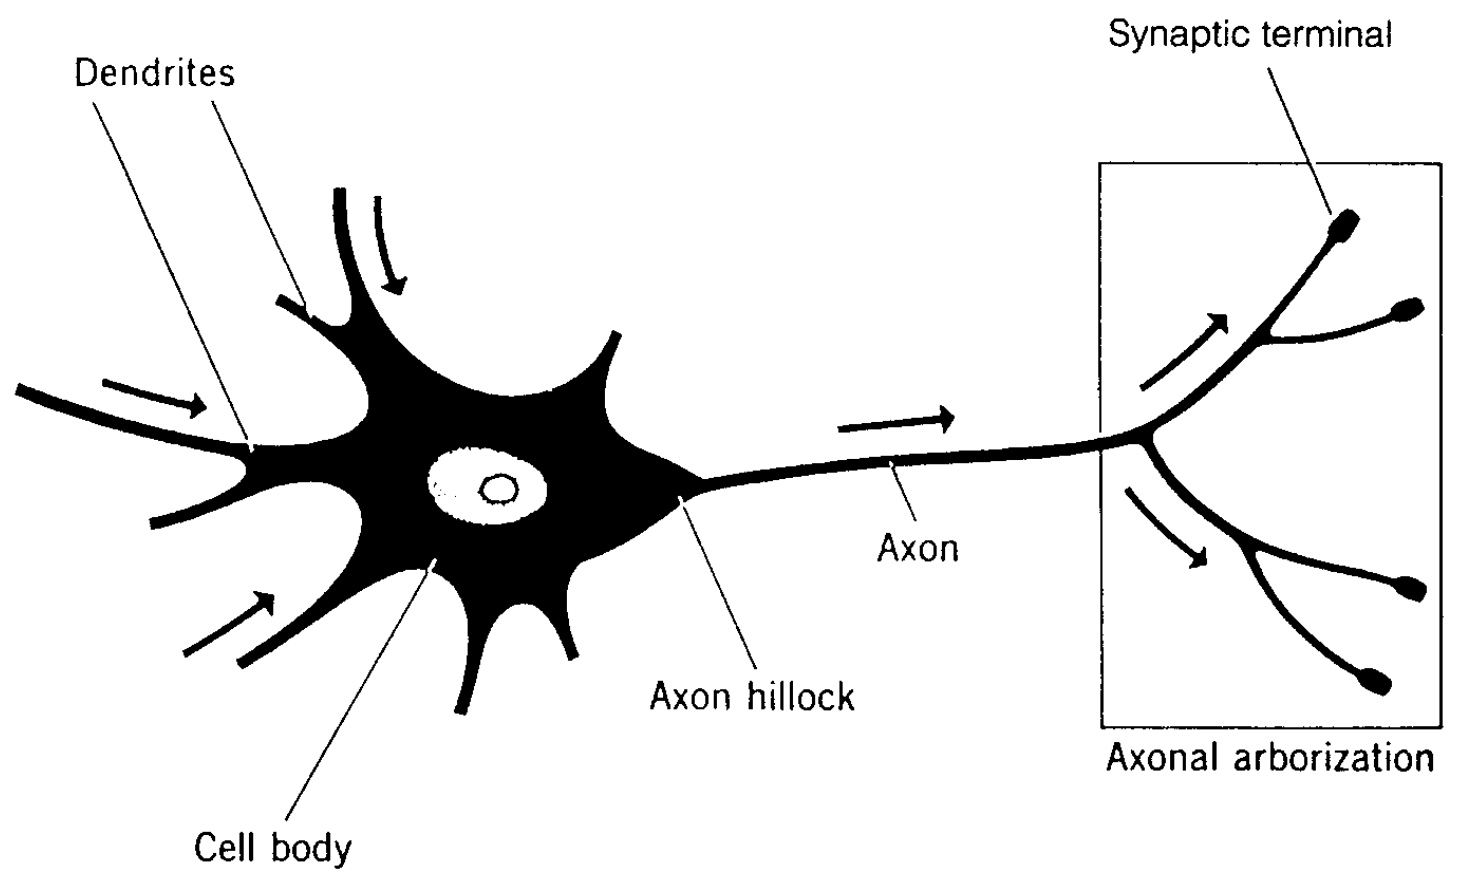
\includegraphics[width=\textwidth]{Figs/neuron.png}
	\label{fig:neuron}
	\caption{Schematic of a neuron. From the caption of the source: \emph{A ``basic neuron'' abstracted from a motor neuron of [the] mammalian spinal cord. The dendrites and soma (cell body) constitute the major part of the input surface of the neuron. The axon is the ``output line''. The tips of the branches of the axon form synapses upon other neurons or upon effectors (although synapses may occur along the branches of an axon as well as at the ends)} \cite[p.\ 52]{arbib1989}.}
\end{figure}

We will transport this conception of a white-box model into software by modelling our artificial intelligence as a collection of loosely coupled components that do not directly call each other but rather communicate by putting messages into and reading from a message space.

\paragraph{Reasoning and emotions.} After this groundwork, we will come back to the large-scale systems, specifically imagination, its relationship to affect, and reasoning. We contend that imagination --- perceiving events that are not happening --- is the antecedent of abstract reasoning, and that they both were gradually evolved from older functionality, rather than either being sui generis. With support from fMRI studies, we conceive of imagination as a re-purposing of sensory perception; the same neural circuitry that had been used for the processing of physical stimuli like sights and sounds came to be used for the processing of those which were internally generated, with specific inhibitory signals prevent the imagined interfering with the real.

The concept of imagination being neurologically related to actual perception implies that emotions play the same role in both --- real as well as imagined situations evoke emotional responses, but whereas real ones influence immediate behaviour, imagined ones chiefly influence planning. Being able to think ahead, to play out scenarios in one's head allows one to effectively ask questions like ``How would I like this?'' and ``Would this be harmful?''. Such questions confer upon organisms the ability to plan and to select beneficial courses of action, but without the need for explicit utility functions; their brains merely re-use their old circuitry in a novel way.

Abstract reasoning, too, is assumed to be an incremental development of pre-existing capabilities: with the ability to simulate physical worlds in place, brains were able to develop the ability to simulate {\em symbolic} ones. The same mechanism that had dealt with the processing of internally generated physical stimuli was employed in the simulation and mental manipulation of things like numbers, glyphs, propositions, or the minds of other individuals.

\paragraph{Toy AI.} The second part of the thesis puts the above considerations into practice. We derive an architecture that is influenced by the work of Minsky \cite{societyOfMind} and Sloman \cite{sloman1993,sloman1997}, as well as of Sander et al. \cite{DBLP:journals/nn/SanderGS05} and Gadanho and Hallam \cite{DBLP:journals/adb/GadanhoH01}. This AI will consist of subsystems for affect, belief generation, decision-making, and perception. For expediency's sake, we will not implement a true white-box model; rather, we will loosely couple the components so that each inserts messages into a common message space, from which other components may take what they desire. While implementing a fundamentally new computational model would be interesting, it would also be beyond the scope of the thesis. Instead, we loosely couple the components: each one will insert messages into a common container from which others may take whatever messages they can interpret.

The affective system will read messages coming from external perception and belief generation, and create emotional responses to them. These, in turn, will be read by the decision-maker and guide its actions. Actions can be external, in which case they cause the agent to act, or internal, in which case they tell the belief generator which possible world to simulate.

In terms of software engineering, our model has similarities, both to the Actor model \cite{hewittActor}, and to publish/subscribe architectures \cite{publishSubscribe} --- although more as a concession to practicality and less because of a similarity to their theories. The theoretical basis of our implementation is the postulate that the components of the brain function as white boxes and that other components may listen in on their activity, so to speak. Since this is diametrically opposed to the traditional idea of the procedure/function as a black box, which nigh every programming language follows, we compromise and model the cognitive structure as a mesh of loosely coupled components communicating via passing. This description is reminiscent to the Actor model developed by Carl Hewitt et al. \cite{hewittActor}, although there are differences\footnote{Although the implementation is not described in the language of the Actor model, a translation into it would be quite easy.}: in the Actor model, the topology of the network may change through the creation of new actors, and messages are always passed from one source to known targets (via addresses). In our model, on the other hand, there is no topology in a strict sense; messages are put into a global message storage and every component is free to consume any message it deems relevant. Senders do not know who will read their output, and consumers do not know the sources. This arrangement can be seen as a particularly loose variant of a publish/subscribe architecture, in which the source and the target of a message are completely unaware of each other, and in which there are no specific channels to which one may subscribe. The only criterion by which messages may be accepted or rejected is their content.

% We also make use of already existing solutions --- specifically answer-set programming and the \acthex\ solver \dlvhex\ \cite{dlvhex}. The internal world simulation of our agents makes use of the non-monotonic reasoning provided by ASP and \acthex.

\paragraph{World and evaluation.} The so constructed toy AIs will be placed in a simple grid environment that was inspired by the Wumpus world \cite{norvig}. This world is populated by a number of agents, Wumpuses who function as predators, plants which provide food that the agents periodically have to consume, gold, which they can pick up and trade with each other, and dangerous chasms that kill any agent that steps into them. In this world, each agent can perceive and do a variety of things: it can see the cells ahead of it to a certain distance, smell the stench of Wumpuses which function as predators, and feel the gust around fatal chasms. It can move around, turn to rotate its sight cone, take the food from plants, attack other individuals, trade items like food or gold, and communicate with fellow agents by sending gestures in the form of arbitrary strings. The environment is so designed that the information available to the agent is minimal: it does not know about the disposition of other agents, the way in which they will interpret its gestures, the global topology of the world, what items other agents have, or any other information to which a real animal in a real environment would not have access.

The aim of this scenario is to test whether the agent architecture is viable at all and, if so, which affective profiles are more successful than others. While each agent works in the same way, they can be parametrised in their emotional reactions to stimuli and thereby exhibit different personalities, in a manner of speaking. 

\paragraph{Structure of the thesis.} The thesis consists of two large segments. The first one is the theoretical argument and empirical data supporting it in Chapter~\ref{ch:preliminaryConsiderations}. It deals with the origin and purpose of neural systems, their evolution (insofar as is known), the components of which they are likely comprised, and how these could have come about. The constituent sections are
	\begin{itemize}
		\item Section~\ref{sec:relatedWork}, describing relevant previous work in the area of artificial intelligence,
		\item Section~\ref{sec:preliminaryBiologicalConsiderations}, containing the general evolutionary story,
		\item and Section~\ref{sec:whiteBoxModel1}, which describes our hypothesized white-box computation model of the cognition of humans.
	\end{itemize}

The second segment begins with Chapter~\ref{ch:componentModel}, wherein we discuss our model in greater detail. Section~\ref{sec:whiteBoxModel2} explains how to represent white boxes as loosely coupled, interacting components and Section~\ref{sec:mathematicalModel} introduces mathematical language to talk about such components in a formal way.

Chapter~\ref{ch:affectiveArchitecture} then deals with subsystems as well as architectural patterns of which we will make use in the implementation. Chapter~\ref{ch:implementation} then specifies the world in which our agents will have to survive, as well as the components and the architecture of our agents itself.

The thesis closes with Chapter~\ref{ch:conclusion}, which contains the the results of our evaluation as well as future work and ideas for improvement.

%The history of AI is marked by vacillations between two paradigms: the biological and the ideal one. These sometimes move closer to each other, and then apart again, due to the fact that they are naturally in tension, yet also inextricably bound together. The biological model, which subsumes the connectionist and the cybernetic ones, seeks to imitate biological organisms on the lowest level; cybernetics, now unpopular, tried to emulate intelligence via feedback loops; connectionism wants to  build complex cognition out of interconnected, simple parts.



%
%Its most famous instance --- neural networks --- and the approach in general, have, time and time again, failed to produce even the rudimentary intelligence we seen in animals. The high hopes of the pioneers of the field that the mathematical modelling of some primitive, biologically inspired computing machinery, cleverly pieced together, could mimic the cognition of humans, were sorely disappointed. Then, after years of lacklustre results, Marvin Minsky published his devastating proof of the theoretical weakness of perceptrons --- a then popular type of neural network --- in his book {\em Perceptrons: An Introduction to Computational Geometry} \cite{Minsky1988}. This led to the abandonment of the approach among AI researchers and, arguably, to the AI winter of the 1970s. In hindsight, we can say that, despite their unimpeachable brilliance, their position in history imposed upon them a fatal naivete and an optimism born from the ignorance of the harrowing complexity of an organ that had been, in one form or another, a good few hundred million years in the making. The idea that neural networks mimicking the smallest-scale structures in the brain and consisting of few thousand nodes, trained over the course of minutes or days, could hope to emulate human intelligence, turned out to be false.
%
%Though it had been developed coterminously with the connectionist approach, the ideal approach came to prominence after the former's disappointments. We can identify it largely with {\em symbolic} computation, whose proponents falls into the two camps (allegedly first identified by Roger Schank): the {\em neats}, who favour provably correct methods, and the {\em scruffies}, who are willing to use whatever works \cite[pp. 421–424]{McCorduck2004}. Both, to some degree, kept a penchant for mathematical formalisms, but they abandoned the goal of re-tracing the workings of biological brains. The neats especially, in an Aristotelian manner, tried to automate how one {\em ought to think}. How humans accomplished their tasks was no longer of importance; only what they accomplished was --- and preferably, that {\em what} was abstract reasoning. Out of this school thought came many applications that have proved very useful: automated planning, in the forward and backward variety; default and common-sense reasoning; answer-set and logic programming; Prolog; knowledge-based systems that assist experts in their decision-making, in a way, informed an uninformed search algorithms. Many of these can now outperform the best humans in specialized tasks. Knowledge-based in medicine now rival doctors in the quality of their diagnoses \cite[p. 592, Table 31-1]{mycin}. Automated driving system can navigate through traffic accident-free \cite{googleCar}. In chess, the greatest human players have trouble keeping up with computers, as Gary Kasparov famous loss to Deep Blue showed in 1997 \cite{deepBlue}. Yet, impressive as they are --- and they are impressive ---, these {\em weak AIs} have not allowed us to piece together the big picture.\footnote{As a side note, it should be said that that the term ``weak AI'' may be unfairly denigrating. Even if we came into possession of human-level strong AI, so-called weak  AIs would still easily outperform it in special areas, just as they outperform humans today.} As good as they are, one would be hard-pressed to call them intelligent in the colloquial sense. As good as any chess program or automated car is, they are still just machines (again in the colloquial sense). It would indeed be absurd to propose that one could exchange one for the other. While Gary Kasparov was able to drive home after his match against IBM's Deep Blue, the notion of ``car'' was not even part of his opponent's conceptual universe. Equally, the control system in Google's self-driving car would not be able to play chess, or assemble a shopping list, read a book, smell, interpret emotions, or do any number of things of which humans and animals are capable.
%
%In recent years, the schism between the biological/connectionist and the ideal/symbolic schools of thought has grown quite pronounced, they are, on a deeper level, joined at the hip. The simple reason for this is that the brain is both a ``messy'' biological organ, and a high-level computation device. It is neither an amorphous mass of neurons, as connectionism models it, nor is it merely a neutral hardware for idealized reasoning, to which the symbolic approach is wont to reduce it. It is both, and in this thesis, I submit that any strong AI must find find a bridge between the two views and integrate them into one whole.
%
%This thought is not new; such a bridge already exists in the form of the {\em integrated approaches}. This vague category comprises things like James Albus's Hierarchical Control Systems \cite{albusHCS}, Rodney Brook's Subsumption Architectures \cite{brooksSubsumption}, Carnegie-Mellon's 4CAPS \cite{4caps}, and, in theory, the architecture laid out in Minsky's The Emotion Machine \cite{emotionMachine}. The chief commonality of these systems is that they proceed from an engineering perspective, not from the mathematical one of symbolic computation, or the biological one of connectionism. Yet, they attempt to combine the high-quality results of the mathematical methods with the dynamism of the biologically inspired systems. It is to this category to which I hope to make a small contribution by proposing that one must not only consider the mind not just as messy, but something worse: as {\em evolved}. I submit that we can best make sense of the seemingly random jumble of features, defects, idiosyncrasies, and quirks of brains by tracing their history. By going through the developments step-by-step, by proposing simple components that came about one by one and grew over time, what is seemingly random and senseless can begin to make sense. By re-creating them, we can hope to create {\em authentic} intelligences --- ones that match biological ones not just in raw processing power, but also in kind.
